\section{Morphing d'images quelconques}
\label{sec:morphing_images}

\paragraph{} Après avoir abordé la morphose dans des cas simples, notamment celui de formes unies simples et courbes, 
nous allons désormais nous intéresser à la morphose d'images quelconques. De ce fait, l'objectif à atteindre est de pouvoir
passer d'une image à une autre de manière fluide, en conservant les caractéristiques de chacune des images, tout en \important{évitant l'effet juxtaposition}.

\begin{figure}[h!]
    \centering
    \begin{subfigure}{0.4\textwidth}
        \centering
        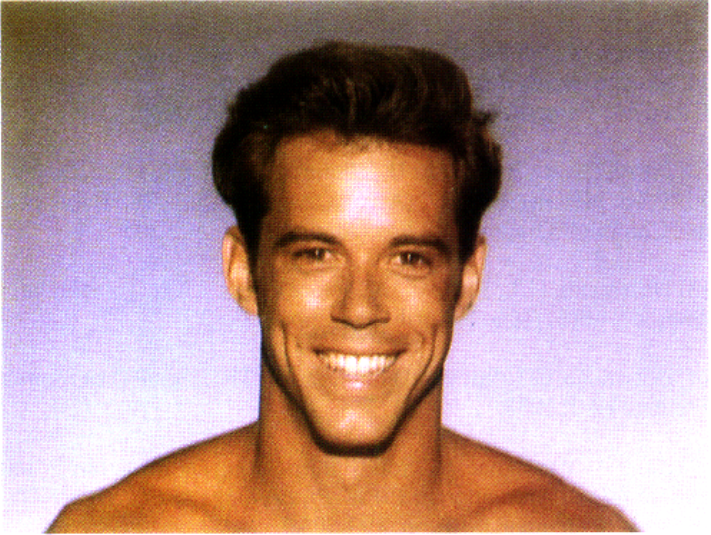
\includegraphics[width=0.8\linewidth]{img/p3/lena.png}
        \caption{Image de départ}
        \label{fig:lena}
    \end{subfigure}
    \begin{subfigure}{0.4\textwidth}
        \centering
        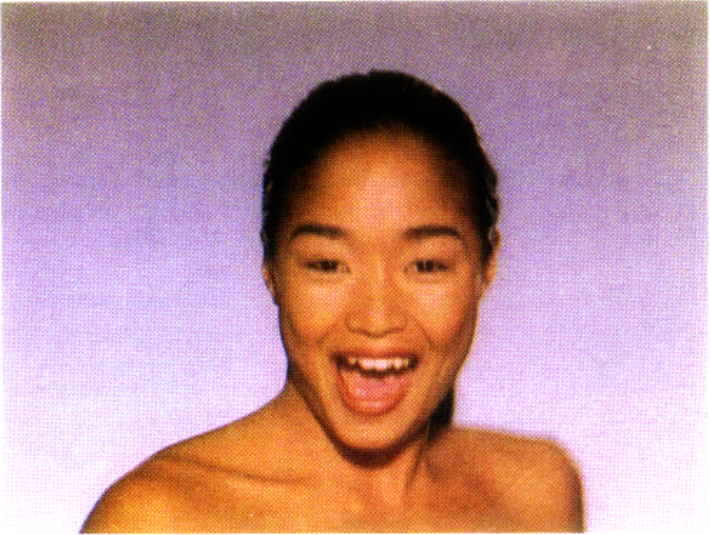
\includegraphics[width=0.8\linewidth]{img/p3/lena2.png}
        \caption{Image d'arrivée}
        \label{fig:lena2}
    \end{subfigure}
    \caption{Paires d'images à morpher \cite{beier1992feature}}
\end{figure}

\paragraph{} Pour ce faire, nous allons nous appuyer sur les travaux de Beier-Nelly \cite{beier1992feature}, qui proposent une méthode de morphing basée sur la paramétrisation de l'image
par des vecteurs de contrôle. Ainsi, chaque pixel de l'image est repéré par une association de positions relatives à ces vecteurs de contrôle. En conséquence de quoi, pour deux images
différentes ayant le même nombre de vecteurs de contrôle, il est possible d'associer chaque pixel de l'une, à un pixel de l'autre (ceci ne signifie pas qu'il existe une bijection entre les pixels des deux images). 

\paragraph{Principe} Le principe de la morphose entre deux images repose sur deux étapes majeures. 
La première consiste à déformer les images de départ et d'arrivée, et la seconde à interpoler les images résultantes.
Ce faisant, il nous est possible d'éviter l'effet de superposition des images. Naturellement, plus le nombre de vecteurs de 
contrôle est élevé, plus la morphose sera précise. De même, un grand nombre d'images intermédiaires permettra d'obtenir
 une animation plus naturelle.

\begin{figure}[h!]
    \centering
    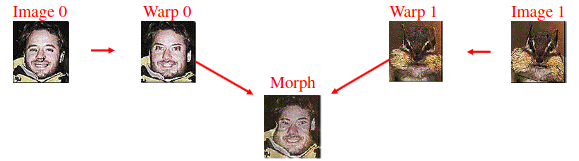
\includegraphics[width=0.8\linewidth]{img/p3/principe.png}
    \caption{Calcul d'un image intermédiaire \cite{CSC320W}}
    \label{fig:morphInter}
\end{figure}

\begin{codeb}
Sur la figure \ref{fig:morphInter}, on peut observer le calcul d'une image intermédiaire \emph{Morph}. 
Explicitement, on a : \couleur{$Morph = (1 - \alpha) \times Wrap_0 + \alpha \times Wrap_1$}, où $\alpha$ est un paramètre variant de 0 à 1.
\end{codeb}

\subsection{Déformation des images}
\label{subsec:deformation}
\subsubsection{Préliminaires}
\begin{definition}
    Soient $P$ une image. On note $w$ sa largeur et $h$ sa hauteur, ainsi que $\mathcal{D}(P)=[0,w]\times[0,h]$.
    On appelle \important{vecteur de contrôle} de $P$ tout couple de points du plan $c=(c_1,c_2)$ tel que $c\in\mathcal{D}(P)$.
\end{definition}

\begin{definition}
    Soient $P$ et $Q$ deux images, ainsi que $p$ et $q$ deux vecteurs de contrôle de respectivement $P$ et $Q$. On définit la
    relation $\sim$ telle que $p \sim Q$ si et seulement si $p$ et $q$ sont appariés. Id est, $p$ et $q$ 
    sont une seule et même entité, mais dans deux contextes (\emph{images}) différents.
\end{definition}
\begin{coder}
    \textbf{Conditions.  } Considérons deux images $P$ et $Q$ à morpher en $N>0$ étapes. 
     Alors, chacune possède $n+1$ vecteurs de contrôle $p_{0},\dots,p_{n}$ et $q_{0},\dots,q_{n}$ tels que pour tout $i \in \{0,\dots,n\}$, $p_{i} \sim q_{i}$.

\end{coder}
\subsubsection{Cas simple: un seul vecteur de contrôle}
\paragraph{Notations.}
Soit $v$ un vecteur de controle et $x$ un point du plan
\begin{itemize}
    \flch On note $v_1$ et $v_2$ les composantes de $v$,
    \flch On note $\widehat{v} = v_2 - v_1 \in\R^2$,
    \flch On note $v^\perp = \frac{\widehat{v}}{\|\widehat{v}\|} \times \begin{pmatrix} 0 & -1 \\ 1 & 0 \end{pmatrix}$,
    \flch On note $d(X,v)$ la distance entre $x$ et la droite passant par la première composante de $v_1$ et portée par $v$.
\end{itemize}

\begin{propriete}
    Soit $c=(P,Q)$ un vecteur de contrôle, $X$ un point du plan, alors :
    \begin{equation}
        \begin{aligned}
            u = \. & \frac{c \cdot (P,X)}{\left\lVert c \right\rVert^2 }
        \end{aligned}
    \end{equation}
    \begin{equation}
        \begin{aligned}
            v =\.  & d(X,c) . v^\perp
        \end{aligned}
    \end{equation}
\end{propriete}
\begin{figure}[h!]
    \centering
    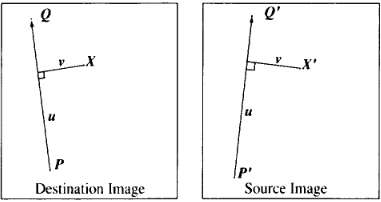
\includegraphics[width=0.6\linewidth]{img/p3/uv.png}
    \caption{Apparaiement à un seul vecteur \cite{beier1992feature}}
    \label{fig:deformation}
\end{figure}
\newpage
\paragraph{Algorithme.} L'algorithme de déformation d'une image avec un seul vecteur de contrôle est donné par l'algorithme \ref{algo:deformation} suivant.
\begin{algorithm}[h!]
    \caption{Déformation d'une image avec un seul vecteur de contrôle \cite{beier1992feature}}
    \label{algo:deformation}
    \KwData{Deux images $D$ et $S$ à morpher, $(P,Q) \sim (P',Q')$ des vecteurs de contrôle de $D$ et $S$ resp.}
    \KwResult{Une image $S$ déformée}
    \For{chaque $X\in\mathcal{D}(D)$}{
    déterminer $(u,v)$\;
    déduire $X'\in\mathcal{D}(S)$ pour ce couple $(u,v)$\;
    }    
    Couleur(X) dans D $\gets$ Couleur(X') dans S\;
    \BlankLine
\end{algorithm}
\subsubsection{Cas général: plusieurs vecteurs de contrôle}
\paragraph{Principe} L'idée est de déformer l'image d'arrivée en fonction des vecteurs de contrôle de l'image de départ.
Pour ce faire, - et à fortiori, bénéficier de l'ensemble des vecteurs de controle - on détermine le barycentre des positions $X'$ calculées dans l'image source
pour chaque vecteur de contrôle. Dans la logique des chose, le poids attribué à chaque ligne doit être le plus fort 
lorsque le pixel est exactement sur la ligne, et diminuer au fur et à mesure que le pixel s'en éloigne.

\paragraph{Poids.} Le poids attribué à chaque ligne est donné par l'équation suivante :
\begin{equation}
    \text { weight }=\left(\frac{\text { length }^p}{(a+\text { dist })}\right)^b
\end{equation}
où \texttt{length} est la longueur d'une ligne. \texttt{dist} est la distance du pixel à la ligne, et \texttt{a, b,} et \texttt{p} 
sont des constantes qui peuvent être utilisées pour modifier l'effet relatif des lignes.\\
\begin{codeb}
    En pratique, nous avons utilisé $a=0.1$, $b=0.5$ et $p=1$ qui ont demblé donné des résultats très satisfaisants. Toutefois, il 
    est essentiel de garder à l'esprit que ces valeurs peuvent être ajustées en fonction des images à morpher et de la sensibilité voulues.
\end{codeb}
\paragraph{Vecteurs de contrôle.} Pour chaque déformation intermédiaire d'ordre $k$, les vecteurs de controles sont déterminés par interpolation linéaire des vecteurs de contrôle de départ et d'arrivée.
\begin{equation}
    \begin{aligned}
        P_{i,k} &= (1-u)P_{i,0} + uP_{i,N}\\
        Q_{i,k} &= (1-u)Q_{i,0} + uQ_{i,N}
    \end{aligned}
\end{equation}
En notant $N$ le nombre d'étapes de la morphose, et $u=\frac{k}{N}$.
\newpage
\paragraph{Algorithme.} L'algorithme de déformation d'une image avec plusieurs vecteurs de contrôle est donné par l'algorithme \ref{algo:deformation2} suivant.
\begin{algorithm}[h!]
    \caption{Déformation d'une image avec deux vecteurs de contrôle \cite{beier1992feature}}
    \label{algo:deformation2}
    \KwData{Deux images $D$ et $S$ à morpher, $(P_i,Q_i) \sim (P_i',Q_i')$ des vecteurs de contrôle de $D$ et $S$ resp.}
    \KwResult{Une image $S$ déformée}
    \For{chaque $X\in\mathcal{D}(D)$}{
    $DSUM \gets (0,0)$\;
    $sommeDesPoids \gets 0$\;
    \For{chaque ligne $(P_i,Q_i)$}{
    déterminer $(u,v)$\;
    déduire $X_i'\in\mathcal{D}(S)$ pour ce couple $(u,v)$\;
    déterminer $D_i = X_i' - X_i$\;
    déterminer la distance la plus courte de $X$ à $(P_i,Q_i)$\;
    déterminer le poids associé à cette distance\;
    $DSUM \gets DSUM + D_i \times poids$\;
    $sommeDesPoids \gets sommeDesPoids + poids$\;
    }
    $X' \gets X + \frac{DSUM}{sommeDesPoids}$\;
    Couleur(X) dans D $\gets$ Couleur(X') dans S\;
    }
    \BlankLine
\end{algorithm}
\paragraph{Exemple.} La figure \ref{fig:mulLi} illustre la déformation de l'image source en image destination, mais surtout la détermination de la 
position $X'$ calculée comme une combinaison linéaire des vecteurs $(X,X_1')$ et $(X,X_2')$ \cite{beier1992feature}.
\begin{figure}[h!]
    \centering
    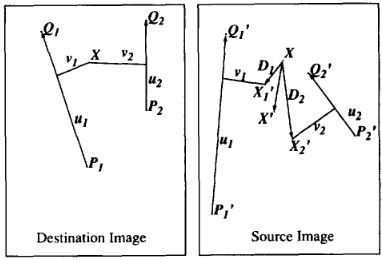
\includegraphics[width=0.8\linewidth]{img/p3/multiple.png}
    \caption{Multiple lignes \cite{beier1992feature}}
    \label{fig:mulLi}
\end{figure}

\subsection{Interpolation des images}
\label{subsec:interpolation}
\paragraph{Principe} L'interpolation des images consiste à déterminer une image intermédiaire entre l'image de départ et l'image d'arrivée.
Pour ce faire, nous avons précalculé des images temporaires, étant pour chacune une deformation judicieuse de l'image de départ et d'arrivée.
Desormais, nous pouvons déterminer une image intermédiaire en interpolant les images temporaires, \ie, en combinant les couleurs des pixels de ces images.

\paragraph{Algorithme.} L'algorithme d'interpolation des images est donné par l'algorithme \ref{algo:interpolation} suivant.
\begin{algorithm}[h!]
    \caption{Interpolation des images \cite{beier1992feature}}
    \label{algo:interpolation}
    \KwData{Deux images $D$ et $S$ à morpher, $N$ le nombre d'étapes de la morphose}
    \KwResult{Une image intermédiaire}
    \For{chaque étape $k$ de la morphose}{
        wrapSrc $\gets$ wrapImage($D$,$S$,$k$)\;
        wrapDst $\gets$ wrapImage($S$,$D$,$k$)\;
        frame $\gets$ \text{Image vide de taille convenable}\;
        \For{chaque $X\in\mathcal{D}(frame)$}{
            $\text{Couleur}_{frame}(X)\gets$ $\gets (1-\alpha) \times \text{Couleur}_{wrapSrc}(X) + \alpha \times \text{Couleur}_{wrapDst}(X)$ $S$\;
        }
    }
    \BlankLine
\end{algorithm}
